\documentclass[a4paper]{iacas}% insert '[draft]' option to show overfull boxes

\usepackage{hyperref}% embedding hyperlinks [must be loaded after dropping]
\usepackage{amsmath}
\usepackage{soul,color}
\usepackage{threeparttable}% tables with footnotes
\usepackage{dcolumn}% decimal-aligned tabular math columns
\newcolumntype{d}{D{.}{.}{-1}}
\usepackage{graphicx}
\usepackage{caption}
\usepackage{subfig}

\title{Computational Fluid Dynamics Modeling of Cathodic Arc Jet}

\author{%
	Anton Ronis\thanks{Gradute Student. E-mail: ro@tx.technion.ac.il}
	\ and
	Igal Kronhaus\thanks{Assistant Professor. E-mail: kronhaus@technion.ac.il}\\
	{\normalsize\itshape
		Faculty of Aerospace Engineering, Technion, Haifa,
		3200003, Israel}
}

% define some commands to maintain consistency
\newcommand{\pkg}[1]{\texttt{#1}}
\newcommand{\cls}[1]{\textsf{#1}}
\newcommand{\file}[1]{\texttt{#1}}

\begin{document}
	
	\maketitle
	
	\begin{abstract}
		In this paper a computational fluid dynamic (CFD) model is developed. A comparison with measurement data is made using spatial distribution of flow parameters as well as a \emph{Taylor-Sedov} blast wave model analysis.
		The numerical solution is carried out using a modified \texttt{OpenFOAM} open source toolbox solver, based on the \texttt{icoFoam} solver. The \texttt{icoFoam} is a pressure based solver for transient incompressible flows which was modified to include an external force field acting on the flow.
		The flow properties -- pressure and velocity qualitatively analyzed in different periods of simulation time. The pressure front position and static values, caused by the jet expansion with respect to time, are sampled and compared to the results obtained from experiment and the \emph{Taylor-Sedov} blast model.
		The CFD jet model of the CAJ predicts well the observed phenomenons from experiments -- \emph{i.e.} forming of an initial cylindrical expansion zone at $1~\mu s$, steady conditions in the CAJ region after around $t = 100~\mu s$, and compatibility with the \emph{Taylor-Sedov} blast model pressure front position and velocity, with respect to time and distance, respectively. 
	\end{abstract}

\section{Introduction}
Active manipulation of flows is an important area of aeronautical research \cite{GADEL}. These devices or actuators promise benefits such as reduction of drag by delaying and/or eliminating separation zones \cite{SIMPSON}. Several examples of flow-control devices include: bumps, vanes (vortex generators), synthetic jets, bleed/suction and plasma actuators.

In contrary to other actuators, plasma actuators can operate on the flow by three different mechanisms \cite{FLOWCTRL}: momentum, shock and chemical effects. Momentum effects induce near surface flow velocities. Shock effects induce very high local gas pressure and temperature which creates gradients in the background air. Chemical effects introduce new species, such as ions, electrons, excited particles into the flow field. The most studied plasma actuator configuration is the dielectric barrier discharge (DBD) which is capable of inducing up to $\sim10$ $m/s$ flows \cite{FLOWCTRL,KOK,WHALLEY,MOREAU}, too low to be effective at high subsonic regimes.

In a recent study \cite{KR}, cathodic arcs operating at atmospheric pressure environment were shown to produce fast jets of gas. This so called cathodic arc jet induce a local flow field velocities of $\ge$ 100 $m/s$ (see Fig. \ref{fig:CAJ}). The jet direction was shown to be controlled by the application of an external magnetic field. Subsequent experiments \cite{KRClose} conducted at different discharge currents suggested the development of a phenomenological model relating the cathode and background gas properties to the observed CAJ. The results suggest the possible use of a CAJ as a flow-control device for external subsonic flows\cite{KRFar}.

\begin{figure}
	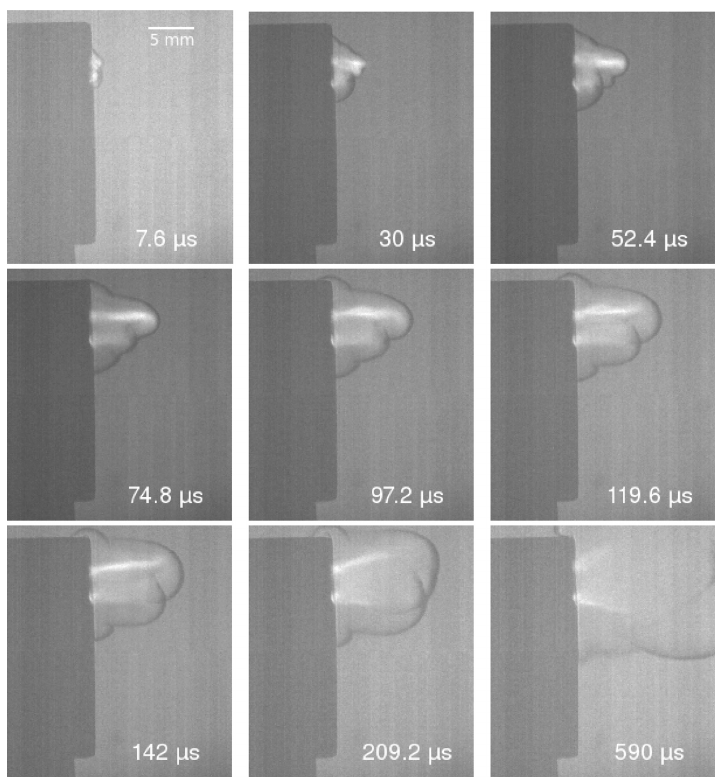
\includegraphics[width=\textwidth]{CAJ_highres.png}
	\caption{Schlieren images of the cathodic arc jet in air. The luminous plasma shows white. The time is counted from the moment of ignition. Reproduced from \cite{KR}.}
	\label{fig:CAJ}
\end{figure}

%In this paper a computational fluid dynamic (CFD) model is developed. A comparison with measurement data is made using spatial distribution of flow parameters as well as a \emph{Taylor-Sedov} blast wave model analysis \cite{TAYLOR,SEDOV}.
%The numerical solution is carried out using a modified \texttt{OpenFOAM} \cite{OPENFOAM} open source toolbox solver, \texttt{forcedIcoFoam} \cite{NS}. The \texttt{forcedIcoFoam} is a pressure based solver for transient incompressible flows modified to include an external force field acting on the flow.
%
%The numerical approach is based on the assumption that the CAJ effect on the background gas can be simulated by an application of acceleration field which causes the gas to reach the velocities obtained in the \cite{KR}. Therefore the jet simulation corresponds to a hot gas expansion at a subsonic speed. Following measurement data \cite{KRClose}, the acceleration field was adjusted to yield a velocity of $500~ m/s$.
%
%The flow properties -- pressure and velocity qualitatively analyzed in different periods of simulation time. Sampling the pressure front position and static values, caused by the jet expansion with respect to time allows one to compare the results obtained from the simulation with \emph{Taylor-Sedov} blast model \cite{TAYLOR,SEDOV}  .
%The pressure front position and velocity obtained in a simulation are visualized in Fig. \ref{fig:model_position} and Fig. \ref{fig:model_velocity}, respectively. The results correspond well with the measured data in \cite{KR}.
%
%The CFD jet model of the CAJ predicts well the observed phenomenons from \cite{KR} -- \emph{i.e.} forming of an initial cylindrical expansion zone at $1~\mu s$, steady conditions in the jet area after around $t = 100~\mu s$, and compatibility with the \emph{Taylor-Sedov} blast model pressure front position and velocity, with respect to time and distance, respectively. Modeling the CAJ as a jet results in some deficiencies -- mainly the addition of mass to the background gas domain and the generation of vortices caused by the flow expansion at the inlet edge. These deficiencies are notable in the local jet domain and must be accounted for in the final CFD model of the CAJ. 
%
%

\section{Physical Model}\label{sec:physical_model}
Observing Fig. \ref{fig:CAJ}, we can divide the formation of a CAJ to two subsequent events:
\begin{enumerate}
	\item Plasma formation in a bounded region
	\item CAJ plume expansion towards the background gas
\end{enumerate}

In the first event a small yet energized volume of plasma particles is generated. This shock boundary is formed in $1~\mu s$ for the given background pressure \cite{meunier1987experimental} and is bounded by a boundary radius which is related to the cathode parameters, discharge current and the background gas. The properties of this boundary radius are discussed in Subsection \ref{subs:boundary_radius}. 

Subsequently, the second event begins with an expansion of the energized volume generated at the discharge core. This expansion is followed by the formation of a jet caused by a momentum and energy transfer of the plasma particles to the gas. It is seen that after the initial boundary expansion certain \textit{steady-state} conditions are met in the jet plume region. The initial expansion and resultant gas jet are discussed in Subsection \ref{subs:CAJ_expansion}. 

\subsection{Plasma-Gas Boundary Radius}\label{subs:boundary_radius}

The force exerted on the plasma particles can be written as:

\begin{eqnarray}\label{eqn:plasma_force}
	F_i &= &\frac{M_i V_i f}{Z e} I_d
\end{eqnarray}

Where $M_i$ is the ion mass, $V_i$ is the ion velocity, $f$ is the ion current fraction, $Z$ is the charge state, $I_d$ is the current magnitude and $e$ is the electron charge.

Constraining an equilibrium of forces between the plasma and gas we can use \eqref{eqn:plasma_force} to express the area, $A$, for a given pressure, $p$, for which an equilibrium is achieved:

\begin{eqnarray}\label{}
	F_g & = & F_i \\\label{eqn:rel_equiv_force}
	p A & = & \frac{M_i V_i f}{Z e} I_d\\
	A & = & \frac{M_i V_i f}{Z e} \frac{1}{p} I_d
\end{eqnarray}

Assuming cylindrical distribution of the gas pressure on the plasma, i.e $A = \pi r^2$, the following expression is obtained for the radius, $r$:

\begin{eqnarray}
\label{eqn:rad_equiv_force}
	r & = & \mathcal{C}\sqrt{I_d}
\end{eqnarray}


Where $\mathcal{C} = \sqrt{\frac{1}{\pi}\frac{M_i V_i f}{Z e}\frac{1}{p}}$ is a constant defined by the cathode and experimental parameters. This allows us to relate the boundary radius $r$ to the discharge current, $I_d$, thus resulting in a simplified relation between the two, for a given set of cathode parameters. By using known cathodic arc parameters for Cu ion in \eqref{eqn:rad_equiv_force}: $p = 101 \times 10^3~\mathrm{Pa}$, ion mass $M_i = 1.055 \times 10^{-25}~\mathrm{kg}$, ion velocity $V_i = 12.5 \times 10^3~\mathrm{m/s}$, ion current fraction $f=0.08$, charge state $Z = 1.8$ and $I_d$ values measured in previous experiments \cite{KR,KRClose} we can calculate the resultant boundary radius, $r$. Results for the given parameters are shown in Table~\ref{t:radii}. 

\begin{table}[hbt]
	\begin{center}
		\begin{threeparttable}
			\caption{Calculated CAJ boundary radius}
			\label{t:radii}
			\begin{tabular}{lc|c}
				Parameter &
				\multicolumn{2}{c}{Value}\\\hline
				$p$ & \multicolumn{2}{c}{$101 \times 10^3~\mathrm{Pa} $} \\
				$M_i$  	& \multicolumn{2}{c}{$1.055 \times 10^{-25}~\mathrm{kg} $}  \\
				$V_i$ 	& \multicolumn{2}{c}{$12.5 \times 10^3~\mathrm{m/s} $}  \\
				$f$ 	& \multicolumn{2}{c}{$0.08 $} \\
				$Z$	& \multicolumn{2}{c}{$1.8 $} \\
				$I_d$  & 230~A & 40~A\\
				$r$ 	& 0.5~mm & 0.2~mm
			\end{tabular}
		\end{threeparttable}
	\end{center}
\end{table}

\subsection{CAJ Plume Expansion Region}\label{subs:CAJ_expansion}

The preliminary effect of the high energized concentration of plasma can be modeled \cite{KR} as a disturbed expansion, corresponding with \emph{Taylor-Sedov} blast wave model \cite{TAYLOR,SEDOV}: 

\begin{eqnarray}\label{eqn:taylor_sedov}
r^5 t^{-2} &=& \mathrm{constant}
\end{eqnarray}

This expansion is measured to begin with a sonic velocity of $\approx 500~\mathrm{m/s}$ \cite{KRClose}, quickly decaying towards $\approx 50~\mathrm{m/s}$ \cite{KR,KRFar} at $\approx 10~\mathrm{mm}$ as visualized in Fig. \ref{fig:CAJ}.

Following the blast expansion is the formation of jet generated at the plasma-gas boundary. This jet is assumed to follow the initial blast expansion velocities close to the boundary while decreasing in velocity with the increase of distance from the boundary. The results summarized in Table~\ref{t:radii} showcase that an equilibrium is achieved for distances of less than 1~mm. We can therefore assume that for farther regions (distances above 1~mm) a decay in the plasma density occurs -- which corresponds to a loss of plasma energy. Assuming a conservation of energy in the plasma-gas spherical region, we can thus expect an increase in the gas' energy, in turn.

We note two main contributors to the generation of the jet inside the CAJ plume expansion zone: thermal -- corresponding to heating the gas thus creating an expanding jet; momentum -- corresponding to momentum transfer from the plasma particles and the gas by elastic collisions. As the jet is formed in a relatively small time-scale, we assume that the larger contributions comes from the momentum transfer due to the typical gas heat dissipation time constants \cite{KRClose}.

Assuming steady state conditions at the boundary, we can express the exerted force on the gas with respect to velocity as:

\begin{eqnarray}\label{eqn:force_mass_flux}
	F_g &=& \dot{m} V_g
\end{eqnarray}

Substituting the mass flux $\dot{m}$ for $\rho V_g A_{o}$ -- where $A_{o}$ represents a circular cross section through which the jet flows and $\rho$ is the fluid density, yields:

\begin{eqnarray}\label{eqn:force_density}
F_g &=& \rho V^2_g A_{o}
\end{eqnarray}

However, we know that the boundary radius defined by an equivalence between the flow's pressure field an the plasma's force. Comparing the former with 
\eqref{eqn:force_density} thus yields:

\begin{eqnarray}\label{eqn:force_gas_equal}
p A &=& \rho V^2_g A_{o}
\end{eqnarray}

Substituting the areas $A$ and $A_o$ with the relevant expressions involving the boundary radius, $r$ results in: 

\begin{eqnarray}\label{eqn:force_gas_ratio}
p \cdot \pi r^2 &=& \rho V^2_g \cdot \pi r^2 \\
\frac{p}{\rho} &=& \frac{V^2_g}{2}
\end{eqnarray}

Using the state equation for an ideal gas, we get:

\begin{eqnarray}\label{eqn:force_gas_temperature}
	T &=& \frac{V^2_g}{R}
\end{eqnarray}

Where $T$ is the temperature and $R$ is the specific gas constant. \eqref{eqn:force_gas_temperature} relates the gas temperature to the jet velocity. We can therefore express the Mach number at the boundary, as:

\begin{eqnarray}
	\mathrm{M} &=& \frac{V_g}{a} \\
	 &=& \frac{\sqrt{RT}}{\sqrt{\gamma R T}}\\\label{eqn:mach}
	 &=& \sqrt{\frac{1}{\gamma}}
\end{eqnarray}

For most cases $\gamma \geq 1$. Specifically for ideal air $\gamma = 1.4$ -- We can therefore conclude that the boundary Mach is $\mathrm{M} = 0.845$

\section{Numerical Model}

The numerical approach is based on the assumption that the CAJ effect on the background gas can be simulated by an application of acceleration field which causes the gas to reach the velocities obtained in the \cite{KR}. Therefore the jet simulation corresponds to a hot gas expansion at a subsonic speed.

The numerical solution is carried out using a modified \texttt{OpenFOAM} \cite{OPENFOAM} open source toolbox solver, based on the \texttt{icoFoam} solver. The \texttt{icoFoam} is a pressure based solver for transient incompressible flows which was modified to include an external force field acting on the flow. An attempt was made to modify the compressible transient solvers \texttt{rhoCentralFoam}, \texttt{rhoPimpleFoam} without success - due to complex flux calculations methods implemented in the solvers. It is therefore important to note that compressibility effects are not taken into account in the proposed Numerical Model. This fact is plausible due to the fact that $\mathrm{M} < 1$ at boundary, as described in Section \ref{sec:physical_model}, Subsection \ref{subs:CAJ_expansion}, but should be taken into account when discussing the velocity profile.

The numerical domain consists of 250 $\times$ 400\footnote{Grid dimensions were obtained by conducting grid size sensitivity runs, analyzing the CAJ profile} grid points representing a 15 mm $\times$ 30 mm dimensioned physical domain. 

We simulate the plasma-gas interaction by assuming a constant acceleration field just beneath the CAJ expansion plume region. The field properties are defined by the cathode spot and background gas parameters, as described in Section \ref{sec:physical_model}, Subsection \ref{subs:boundary_radius}. For the observed parameters representing the experiment \cite{KR} of Fig.~\ref{fig:CAJ}, the field was placed at $ y < 0.5~ \mathrm{mm} $ at a width of $r = 1~\mathrm{mm}$ (Fig. \ref{fig:force_field}), centered around $x=0~\mathrm{mm}$. This corresponds to a discharge current of around 230 A.

\begin{figure}[htbp]
	\centering
	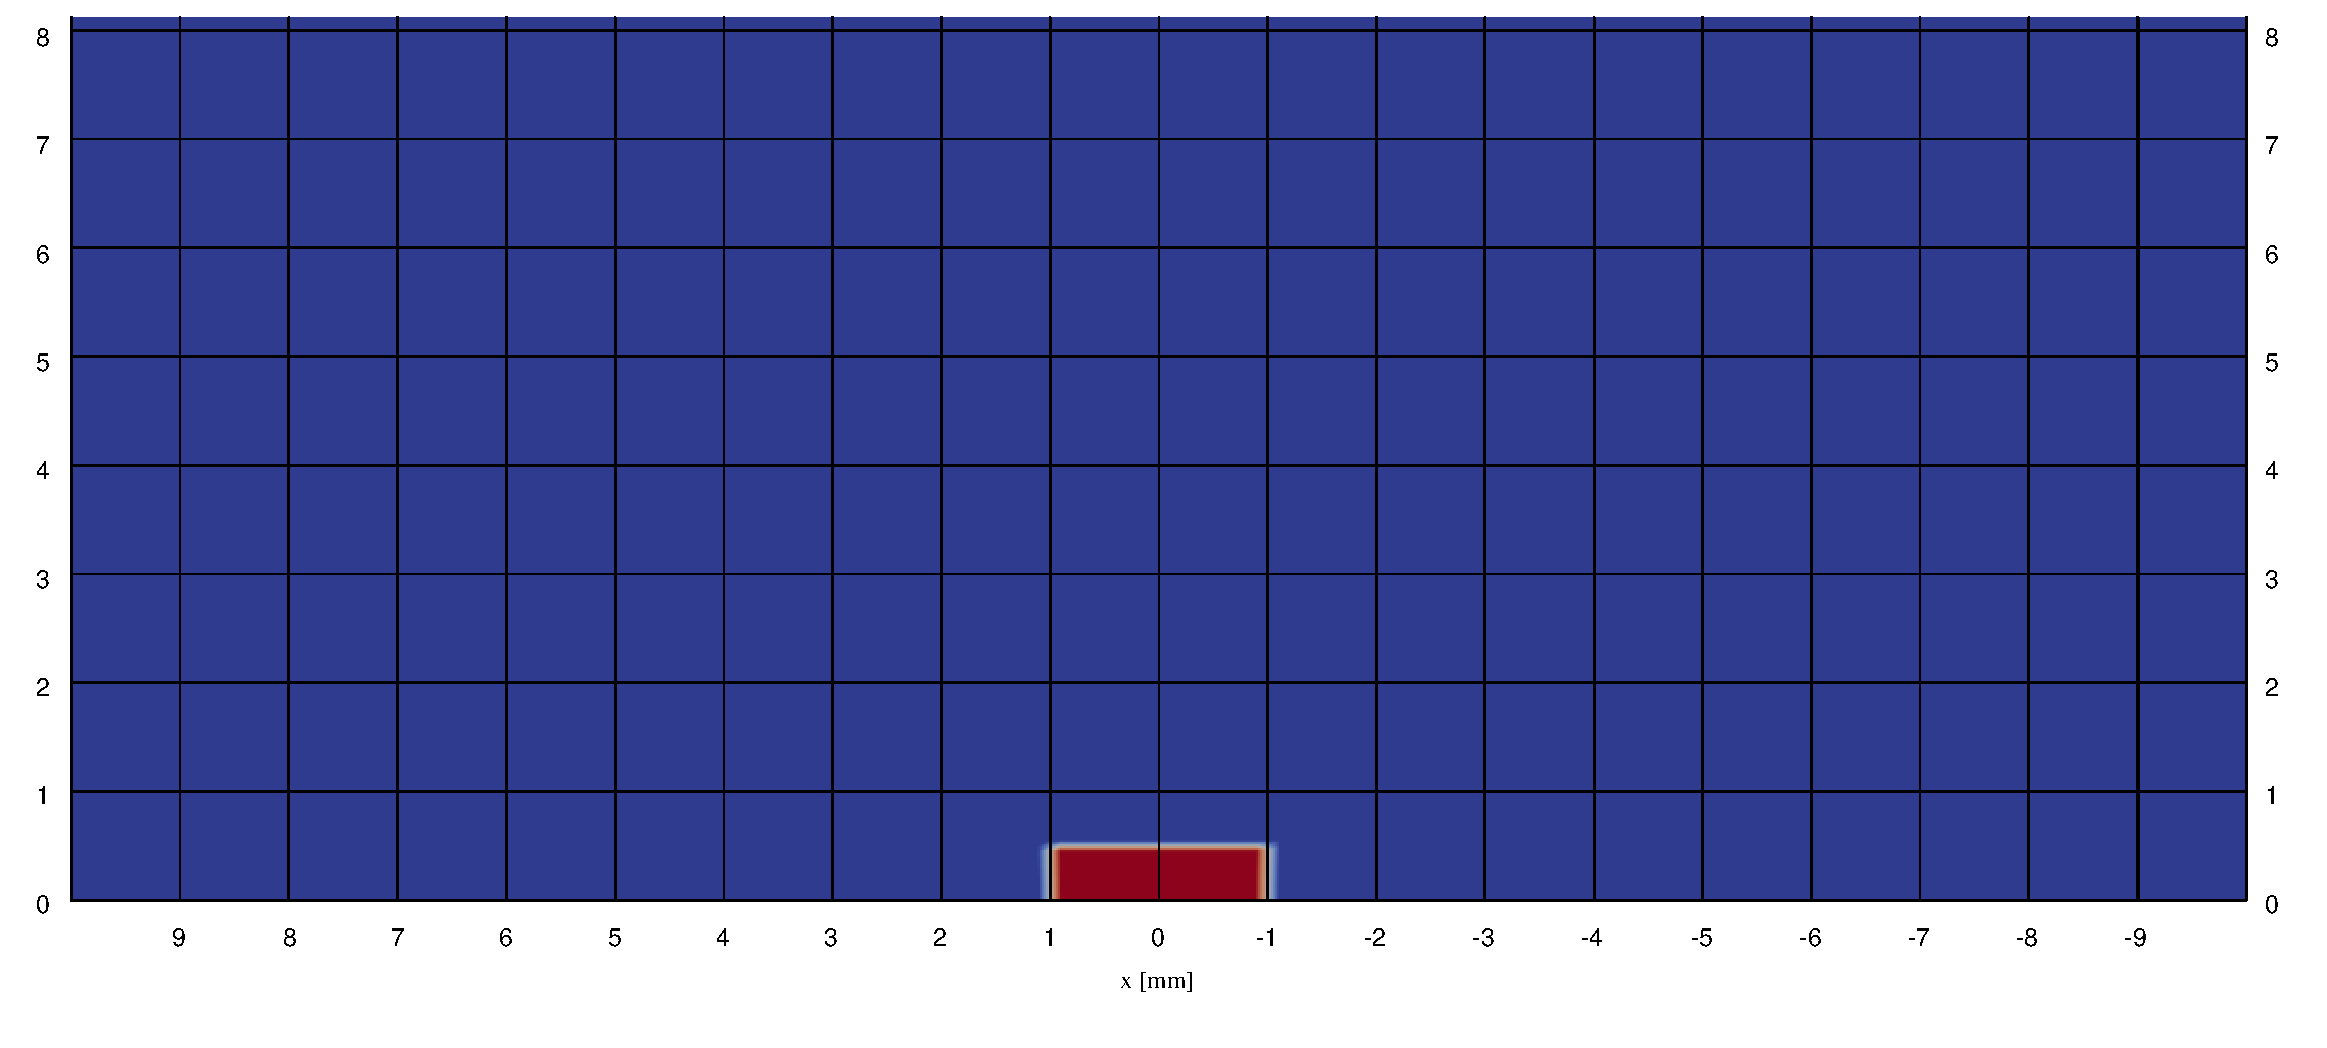
\includegraphics[width=0.9\textwidth]{forceField}
	\caption{Force field representation in the numerical domain. Red zone corresponds with the added acceleration field}\label{fig:force_field}
\end{figure}

Following measurement data \cite{KRClose}, the acceleration field is adjusted to yield a velocity of $500~ m/s$. It is assumed that the discharge current affects the observed initial CAJ expansion velocity location, yet not the value itself, which in turn defined by the background gas properties \cite{KR,KRClose,KRFar}. The gas is assumed to be motionless, atmospheric at a room temperature. The added momentum resulted from the acceleration field is translated to an expansion of the gas in the form of a jet.

\section{Results \& Discussion}

The simulation is executed at a modified time step  constraining a Courant number, $\mathcal{C} \leq 0.1$, for a total simulation time of $t = 500~\mu s$. The solution is depicted at the numerical domain region corresponding with the CAJ plume expansion region ($ y > 1 \mathrm{mm} $). 

The velocity and pressure fields obtained at $ t = 500~\mu s $ are illustrated in Fig. \ref{fig:velocity_field} and Fig. \ref{fig:pressure_field}, respectively. The acceleration field results in the formation of a time evolving jet that reaches pseudo-steady-state conditions by $t = 500~\mu s$.

The pressure front position and velocity obtained in a simulation are visualized in Fig. \ref{fig:model_position} and Fig. \ref{fig:model_velocity}, respectively. There's a very good correspondence between the Taylor-Sedov \cite{TAYLOR,SEDOV} Blast model and the pressure/velocity front velocities obtained in the simulation. A comparison between the measurements from \cite{KR} shows as well similar behaviors for the velocity front evolution with time.

The pressure front velocity and the CAJ velocity profile evolution are depicted in Fig. \ref{fig:model_caj_velocity}. We see that even though the velocity profile developed in the CAJ  follows the pressure's front velocity behind, the former one is larger in magnitude. This phenomenon corresponds well with the constant mass flux assumption yielding higher speeds at higher temperature regions obtained inside the CAJ region relative to lower speeds obtained at lower temperature obtained at the CAJ boundary with the background gas. However, these two velocities converge as the CAJ temperature drops towards the boundary with the background gas. 

\begin{figure}
	\centering
	
	\subfloat[Velocity]{
		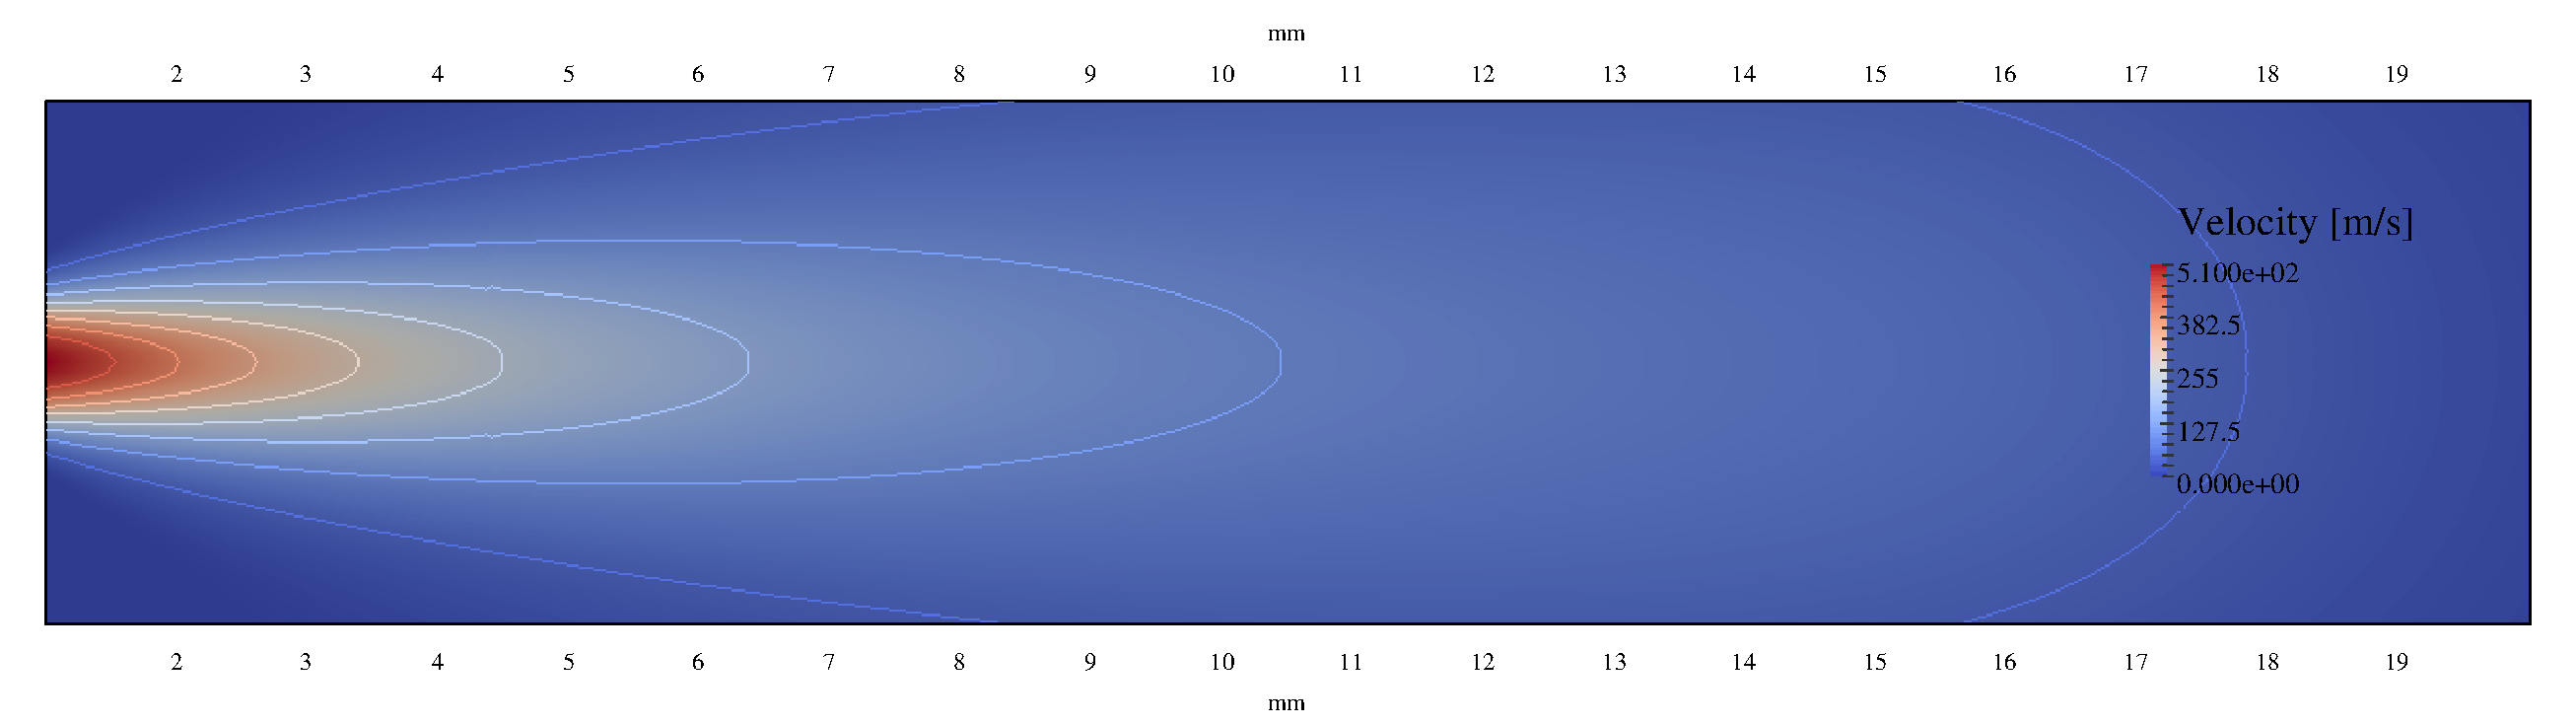
\includegraphics[width=1\textwidth]{velocityField}
		\label{fig:velocity_field}
	}
	
	\subfloat[Pressure]{
		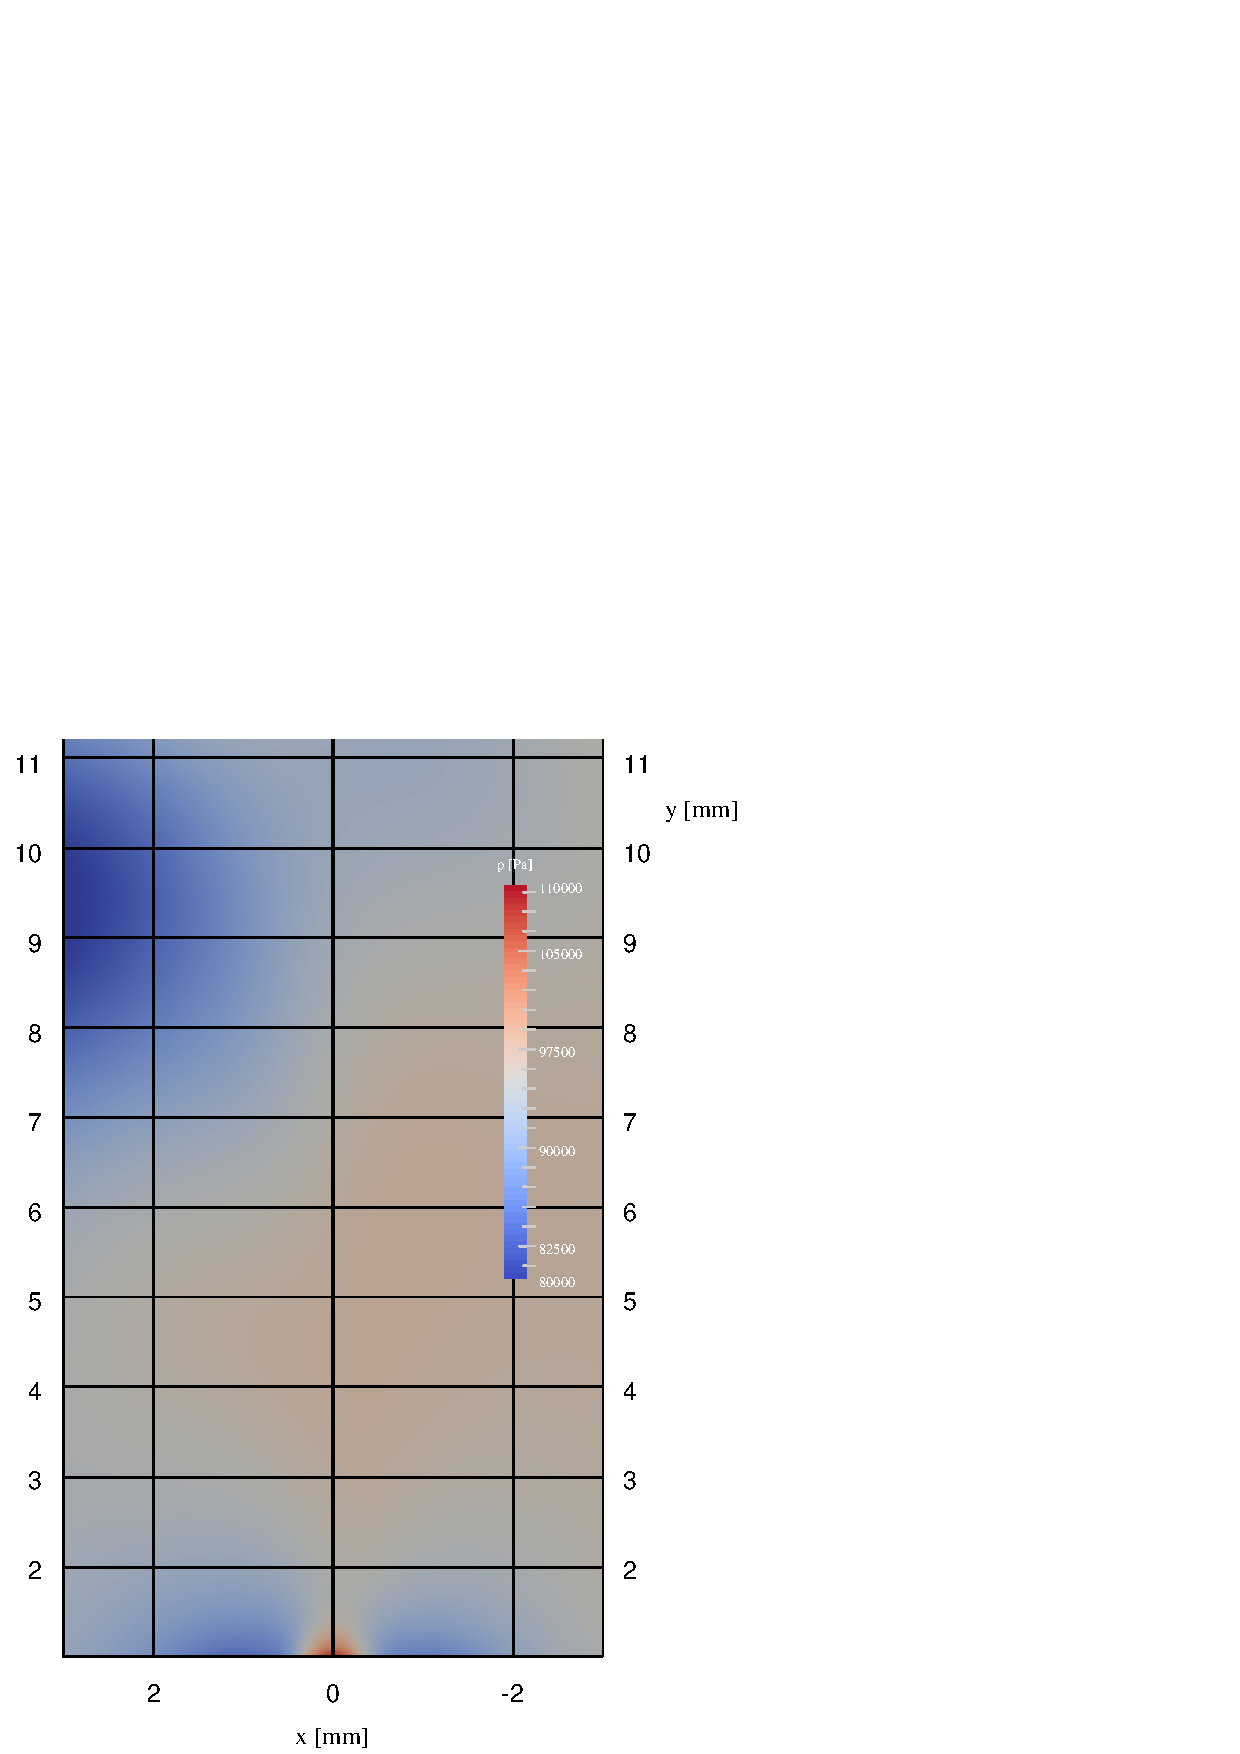
\includegraphics[width=1\textwidth]{pressureField}
		\label{fig:pressure_field}
	}
	\caption{(a) Velocity field, $ t = 500~\mu s $; (b) Pressure field, $ t = 500~\mu s $}
\end{figure}

\begin{figure}
	\subfloat[Position]{
		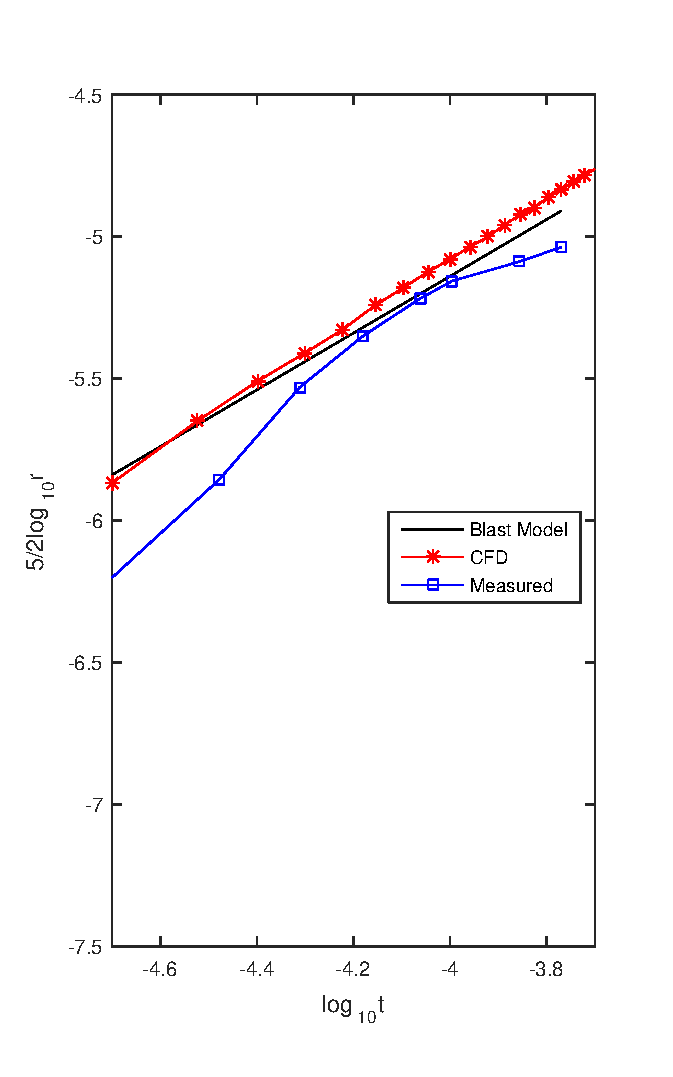
\includegraphics[width=0.5\textwidth]{ModelJetPosition.eps}
		\label{fig:model_position}
	}
	\subfloat[Velocity vs. Position]{
		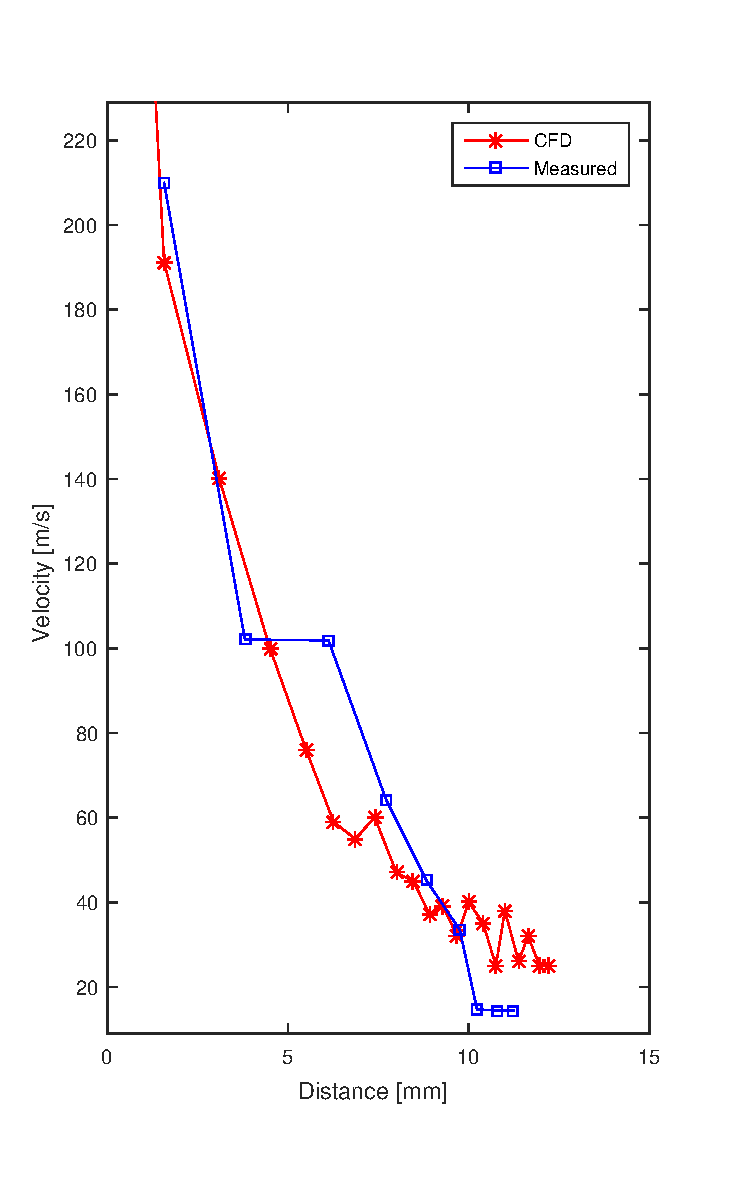
\includegraphics[width=0.5\textwidth]{ModelJetVelocity.eps}
		\label{fig:model_velocity}
	}
	\caption{(a) Time evolution of gas pressure front position (squares - experiment, stars - CFD) together with a linear fit of the blast wave model (black line); (b) the gas pressure front velocity versus position, measured in the direction of the plasma jet (squares) together with the computed CFD velocity of the front (stars). Experiment data reproduced from \cite{KR}}
	\label{fig:model_blast}
\end{figure}

\begin{figure}
	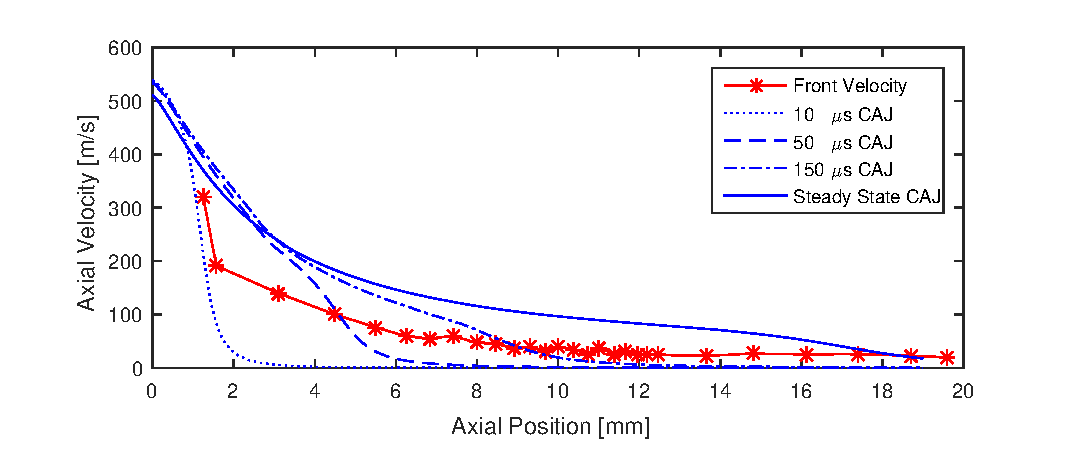
\includegraphics[width=\textwidth]{Vel_Times.eps}
	\caption{Front expansion rate (red squares); Time evolution of the CAJ velocity profile for sample times of $10~\mu s$, $50~\mu s$, $100~\mu s$, $150~\mu s$ and Steady state conditions (bline line); $50~m/s$ boundary line (black dash) }
	\label{fig:model_caj_velocity}
\end{figure}

\section{Conclusions}
A computational fluid dynamic (CFD) model is developed and compared with measurement data by using spatial distribution of flow parameters as well as a \emph{Taylor-Sedov} blast wave model analysis.
A modified \texttt{OpenFOAM} open source toolbox solver, based on the \texttt{icoFoam} solver was modified to include an external force field acting on the flow, simulating the acceleration of the background gas due to the plasma source.
The flow properties -- pressure and velocity were qualitatively analyzed in different periods of simulation time and showed a good corresponds with the measurements obtained at \cite{KR,KRClose,KRFar} (See Fig. \ref{fig:CAJ}). The pressure front position and static values, caused by the jet expansion with respect to time, were sampled and compared to the results obtained from experiment and the \emph{Taylor-Sedov} blast mode and showed a good correspondence between the results (See Figs. \ref{fig:model_position},\ref{fig:model_velocity}).
All in all, the CFD jet model of the CAJ predicts well the observed phenomenons from experiments -- \emph{i.e.} forming of an initial cylindrical expansion zone at $1~\mu s$, steady conditions in the CAJ region after around $t = 100~\mu s$, and compatibility with the \emph{Taylor-Sedov} blast model pressure front position and velocity, with respect to time and distance, respectively. Further studies are to be conducted analyzing the effects of cross-flow background gas \cite{KRClose} on the CAJ based on the suggested implementation of the model.

\clearpage
\bibliography{bibtex_database}
\bibliographystyle{iacas}
\end{document}


%%% Local Variables:
%%% mode: latex
%%% TeX-master: t
%%% End:
